\begin{figure}[t]
\centering
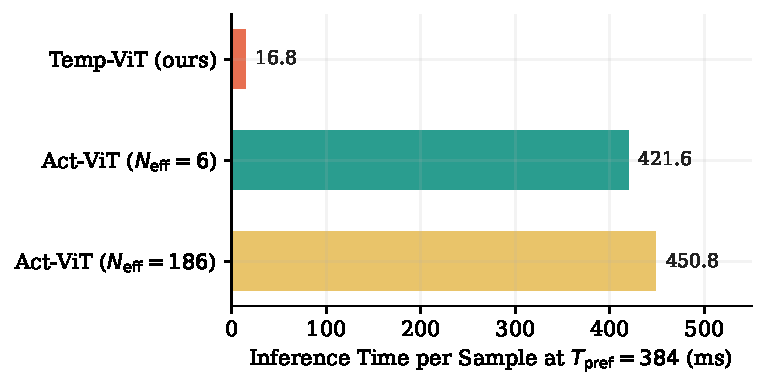
\includegraphics[width=0.95\linewidth]{figs/fig_inference_time.pdf}
\caption{Wall-clock time to score every token of one $T = 384$-token
LongFact passage on a single H200, batch~1, FP32. ACT-ViT emits one
scalar per call, so labelling every token requires $T$ sequential
forwards; per-call latency is small but the total scales linearly with
the response length, even when the post-pool ViT input is widened to
recover long-range accuracy (\emph{N\textsubscript{eff}=186}).
Temp-ViT produces the full per-token logit vector in a single forward
pass and is roughly $25\times$ faster on this passage, illustrating
the real-time-cost weakness of activation-tensor methods that need one
call per generated token.}
\label{fig:inference_time}
\end{figure}
